\documentclass[a4paper,12pt]{article}  % or "report" for larger documents

\usepackage{polski}  % Polish language support
\usepackage[utf8]{inputenc}  % UTF-8 encoding
\usepackage{amsmath, amssymb}  % Math support
\usepackage{float}
\usepackage{graphicx}  % Insert images
\usepackage{hyperref}  % Clickable links
\usepackage{biblatex}  % Bibliography management
\addbibresource{references.bib}  % Reference file
\renewcommand{\figurename}{rys.}

\title{Zadanie konkursowe, eliminajce:\\ Strefa zgniotu}
\author{
  Milosz, Tesiorowski\\
  \and
  Maksymilian Borowy\\
  \and
  Milosz Medwid\\
  \and
  Franciszek Fabinski\\
}
\date{\today}

\begin{document}

\maketitle  % Generates title page

% Wymagania i punktacja:
% 
% Zrozumienie działania strefy zgniotu – 30 pkt.
% Kreatywność i innowacyjność – 30 pkt.
% Estetyka dokumentacji – 20 pkt.
% 
% im fajniejsze beda foty tym lepiej wyjdziemy

\section{Autorska koncepcja}
Nasz projekt strefy zgniotu opiera sie na zalozeniu, ze
auta RC sa dosc lekkie i nawet przy predkosci maksymalnej
raczej nie zegna na przedzie potencjalnego auta,
nie jak samochody wazace ~1 tone. 

Z tego powodu postanowilismy skupic na zginaniu materialu a nie
na jego rozrywaniu.

\begin{figure}[H]
  \centering
  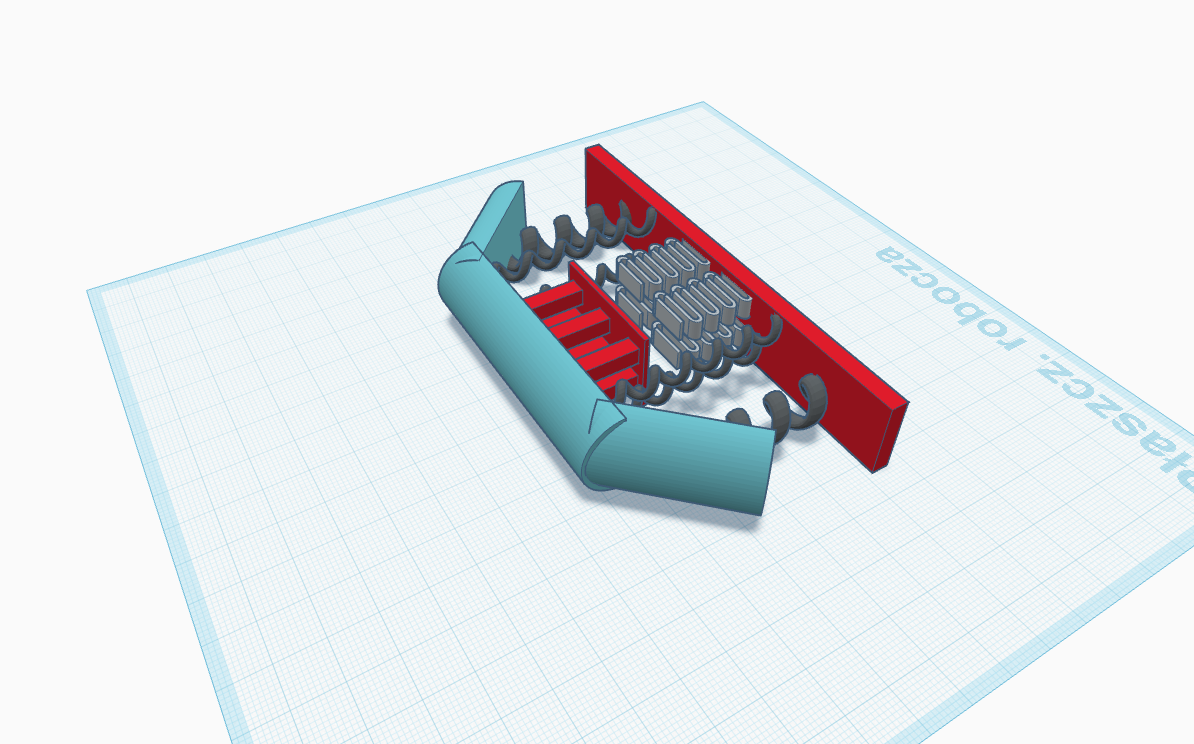
\includegraphics[width=0.95\textwidth]{./pictures/pic1.png}
  \caption{Projekt strefy zgniotu}
\end{figure}


\subsection{Przednia oslona (jasnoniebieska część) - zderzak deformowalny}

Ten element to zderzak pochlaniajacy energię, jego wygięty ksztalt i wysuniecie
do przodu sprawiaja, ze to pierwsza linia kontaktu przy uderzeniu.
Pełni funkcję rozproszenia siły uderzenia i
jej wstępnego pochłonięcia, co odpowiada rzeczywistej zewnętrznej strefie zgniotu.

\subsection{Spiralne elementy (ciemnoszare) – Struktura kontrolowanego zgniotu /
sprężystość}
Elementy te zostały zastosowane ze względu na naturę pojazdów RC. W przeciwieństwie do
klasycznego samochodu, samochodzikiem zdalnie sterowanym często uderzamy w ściany,
wpadamy w niekontrolowane poślizgi, czy zderzamy się z innymi autami. Nie można w takiej
sytuacji pozwolić sobie na wymianę całego elementu zderzaka przy najmniejszym zderzeniu. Stąd
zastosowane sprężyny, które idealnie zamortyzują małe „stuknięcia” pozostawiając w
nienaruszonym stanie elementy stale deformowalne.

\subsection{Moduł centralny (czerwony) – Ramowa ochrona rdzenia}
Czerwony element to usztywniony rdzeń konstrukcyjny, jednocześnie stanowi bazę całej strefy
zgniotu i zamyka modularną konstrukcję.W tym kontekście pełni funkcję niewzruszonej struktury
nośnej, na której zatrzymuje się energia zderzenia. To właśnie w tym miejscu można zamontować
strefę do samochodzika.

\subsection{Blok szarych struktur – Wypełnienie pochłaniające}
To moduł pochłaniający (pasywny tłumik energii) – zaprojektowane na podobę plastrów miodu czy
specjalnie ułożonych kompozytów w autach sportowych. Ze względu na ułożenie spiral, służy
jako główny element rozpraszający energię, jest sercem całej strefy zgniotu. To właśnie ta sekcja
ma przyjąć największą energię podczas zderzenia, sama ulec zniszczeniu, pozostawiając przy tym
nienaruszoną resztę konstrukcji samochodu.

\section{Dobór materiałów}

Chcemy, żeby taki element mógł być dostępny dla każdego, dlatego proponowane przez nas
materiały to typowe filamenty drukarek 3d. Takie „open-sourcowe” podejście ułatwia dostęp do
elementu i zwiększa jego użytkowość.

\subsection{Przednia osłona: **TPU**}
umożliwia wydrukowanym konstrukcjom odkształcanie się i
powracanie do pierwotnego kształtu. Jest to materiał elastyczny, odporny na uderzenia,
świetnie absorbujący energię. Idealny do elementów sprężystych, które mają się zgniatać i
wracać do formy.

\subsection{Czerwone elementy: **ABS**}
wydruki, które powstają z tego filamentu charakteryzują się dużą
twardością i udarnością. Są także bardziej odporne na wysokie temperatury i zarysowania. Do
tego, można go obrabiać – np. szlifować, wiercić, kleić.

\subsection{Jasnoszara sekcja - **PLA**}
Stworzone z ekologicznego materiału, łatwe w druku i zapewniaja wysoką
jakość. Sam w sobie materiał jest dość kruchy, co pozwoli na dobre rozprowadzenie energii w
ważnym miejscu, jednocześnie jest najłatwiejszy do samodzielnego wydruku, co pozwoli
potencjalnym użytkownikom jego szybką wymianę.

\subsection{Ciemnoszare sprężyny - **Stal nierdzewna lub sprężynowa**}
zastosowanie sprężyn typowych
dla tego typu konstrukcji to pewny i sprawdzony wybór od lat stosowany w modelarstwie. Stąd
elementy te są bardzo łatwo dostępne, a również pozwalają na „dostrojenie” strefy zgniotu,
zależnie od dobranego rodzaju.

\section{Uzasadnienie wyboru konstrukcji}

Nasze rozwiązanie dobrze naśladuje sposób, w jaki działa strefa zgniotu w rzeczywistych
samochodach:
\smallbreak
Energia kinetyczna uderzenia nie trafia od razu do "kabiny" (czyli wnętrza modelu RC), tylko jest
pochłaniana warstwowo. Zastosowanie spiralnych elementów (sprężynujących), zderzaka i
sztywniejszego rdzenia imituje układ: elastyczna powłoka – strefa deformowalna – struktura
nośna. To zwiększa realizm działania i bezpieczeństwo komponentów wewnętrznych.
\smallbreak
Spirale jako kontrolowane elementy deformacyjne:
\smallbreak
Zastosowanie spiralnych struktur (lub sprężyn) to idealne podejście do RC ponieważ pochłaniają
energię uderzenia sprężyście, bez trwałych uszkodzeń – model może dalej jeździć. Można je łatwo
wymienić lub dostosować twardość do różnych warunków (np. różnych torów, prędkości).
Działają modułowo – nie trzeba projektować całej strefy od nowa po wypadku.
\smallbreak
Ochrona kluczowych elementów modelu RC:
\smallbreak
Z tyłu umieszczony został sztywny rdzeń, który nie ulega odkształceniu. Spirale i przednia strefa
zgniotu chronią elektronikę, silnik lub baterię, działając jak strefa pochłaniająca uderzenie i bufor,
który zapobiega przenoszeniu całej siły na delikatne elementy. To przedłuża żywotność ważnych i
drogich części.
\smallbreak
Możliwość testowania i regulacji:
\smallbreak
Nasze rozwiązanie można łatwo modyfikować (zmieniać twardość, kształt spirali, infill, długość
elementów), testować w warunkach zbliżonych do rzeczywistych, a co najważniej


\printbibliography

\end{document}

